% \vspace{-40pt}

\section{Introduction}
\label{sec:intro}

Ensuring the authenticity and provenance of digital visual content is increasingly critical as AI-generated media becomes more prevalent. Traditional watermarking methods have limited robustness to everyday transformations and raise security concerns if models are distributed for local use. C2PA~\cite{c2pa2023} does not work in practical scenarios, due to the signature becoming invalid upon any image transformation. Proof of transformation helps maintain validation after image edits~\cite{vimz, veritas}, but we do not expect many image editors to integrate this technology. To tackle these challenges, we introduce a three-part framework aimed at secure and reliable content provenance detection for AI-generated content in real world.

First, we introduce a perceptual hashing algorithm based on DINOV2 \cite{oquab2023dinov2}, a feature extraction network, that captures the semantic and structural features of images, providing an alternative to watermarking by remaining resilient to common image transformations. Second, to secure the integrity of the provenance detection process, we employ Mutli-Party Fully Homomorphic Encryption~(MP-FHE)~\cite{mouchet2021multiparty}, which allows operations on encrypted data, enabling secure, privacy-preserving computations without compromising the system's security regarding data leakage \cite{gentry2009fully}. Lastly, we extend prior work in AI-generated content detection by training a state of the art model to identify and distinguish AI-generated images directly, in case images are not found in our database.

Deep watermarking algorithms embed a nearly invisible hash into an image, which can later be extracted using a specialized network to verify and match images~\cite{deep_watermark}. The main objectives of watermarking are~(a)~robustness against natural image distortions and~(b)~minimal alteration of the original image. Most deep watermarking papers report remarkable results on simple spatial distortions such as brightness or contrast, cropping, and flipping. However, they often fail when exposed to destructive frequency-domain transformations, including blurring, JPEG compression, screenshots, and other non-differentiable processes. This limitation arises because watermarking methods embed information in an image’s high-frequency components, which are often degraded via compression during everyday manipulations like social media uploads~\cite{laghari2018assessment}, sharing on messaging apps~\cite{anwar2021image}, format conversions, resizing, and embedding in videos~\cite{YoutubeCompression}, making watermarking ineffective for content provenance detection in practical settings. 

Traditionally, watermarking requires training a separate deep-learning model to embed watermarks into an image, making them easily removable. However, Meta's recently developed framework, Stable Signature~\cite{meta2023stablesig}, integrates watermarking directly into the diffusion model through fine-tuning, eliminating the need for an additional model during inference. While this approach reduces inference costs, it introduces the burden of maintaining a unique set of model weights for each user. Given that the number of customers of diffusion models is in millions, this storage requirement renders the approach impractical for large-scale industry deployment unless the model is provided to users for local inference. However, as the authors demonstrated, releasing the model to users introduces vulnerabilities due to aversion techniques like model purification and collusion, undermining the security and purpose of the watermarking system.

Additionally, watermarking methods might introduce unwanted visible artifacts \cite{waves}. In contrast, perceptual hashes offer a potential alternative. Instead of embedding data, perceptual hashing derives a hash from the image’s semantic embeddings and structural features, which remain largely unaffected by common transformations, making it more suitable for content provenance applications \cite{phash2020}.

%-------------------------------------------------------------------------
After generating perceptual hashes, it's crucial to query them privately to protect sensitive information. For example, closed-source content generators~(such as OpenAI or Canon) should be able to store perceptual hashes of user-generated images in a public database without leaking information that could lead to prompt reconstruction. Likewise, users need to query the database without revealing all of their images to the content provider. Several systems have been developed to address this private approximate nearest neighbors search~(ANNS/PNNS) challenge, including Janus~\cite{edalatnejad2024janus} and Worldcoin's Iris~\cite{iris-search} matching system, Apple's Wally~\cite{wally-search}, and Panther~\cite{li2024panther}.
The Worldcoin Iris Matching system uses secure multiparty computation~(MPC) to perform privacy-preserving fuzzy matching of iris hash codes, which are similar to our proposed perceptual hashes. It operates under a non-collusion assumption between servers to ensure privacy. In contrast, Apple's Wally system introduces differential privacy by adding fake queries to hide the original query, and querying clusters of data rather than the entire database, thus trading off some accuracy for enhanced performance. Wally uses Somewhat Homomorphic Encryption~(SHE) for secure lookups, based on the BFV~\cite{fan2012somewhat, brakerski2012fully} and BGV~\cite{brakerski2014leveled} schemes, which allow a single entity to decrypt any ciphertext without restriction. In contrast, our system is built on a more advanced FHE scheme, Multi-party FHEW~(MP-FHE), which requires multiple parties to participate in decryption~\cite{mouchet2021multiparty, lee2023efficient}. This enables the design of PNNS systems with stronger security guarantees, ensuring that no single entity can access plaintext data without the consent of all other parties.
\begin{figure*}[!t]
    \centering
    \clearpage
    \includegraphics[page=2, width=0.9\linewidth]{proteus.pdf}
    \caption{\textbf{Deep neural feature extractor architecture}. The pipeline consists of a feature extractor network and Locality Sensitive Hashing~(LSH) step. The PCA whitening ensures that all components of the feature vector are uncorrelated so that the hashes of two random different images have the least probability of being the same.}
    \label{fig:perceptual_hash}
\end{figure*}
Modern tools and open-source models have democratized access to synthetic image generation. In this reality, it is unreasonable to expect every image appearing on the internet to be hashed and stored in a registry by some content-producing organization~(CPO) like cameras or AI image APIs. So, we also build a purely deep learning-based detector to perform the binary classification task of detection of synthetic images.

\noindent In conclusion, we have four main contributions:
\begin{compactenum}
    \item A deep perceptual hashing algorithm that is robust to a wide range of image transformations.
    \item A novel approach to fine-tune any deep-learning-based perceptual hashing model to be adversarially robust. Although several works explore adversarial attacks against perceptual hashing models, to the best of our knowledge, we are the first to introduce an adversarial training mechanism for them.
    \item A cryptographic matching system that privately looks up the provenance of a perceptual hash in a registry, without leaking any data about the registry items or the queried perceptual hash.
    \item A deep learning based detector to detect synthetic images that are not stored in the registry.
\end{compactenum}
